\chapter{Project Idea}
\section{Problem Domain}
We defined in our opinion the most important domains which a Reverse Engineer has to have knowledge of. \\
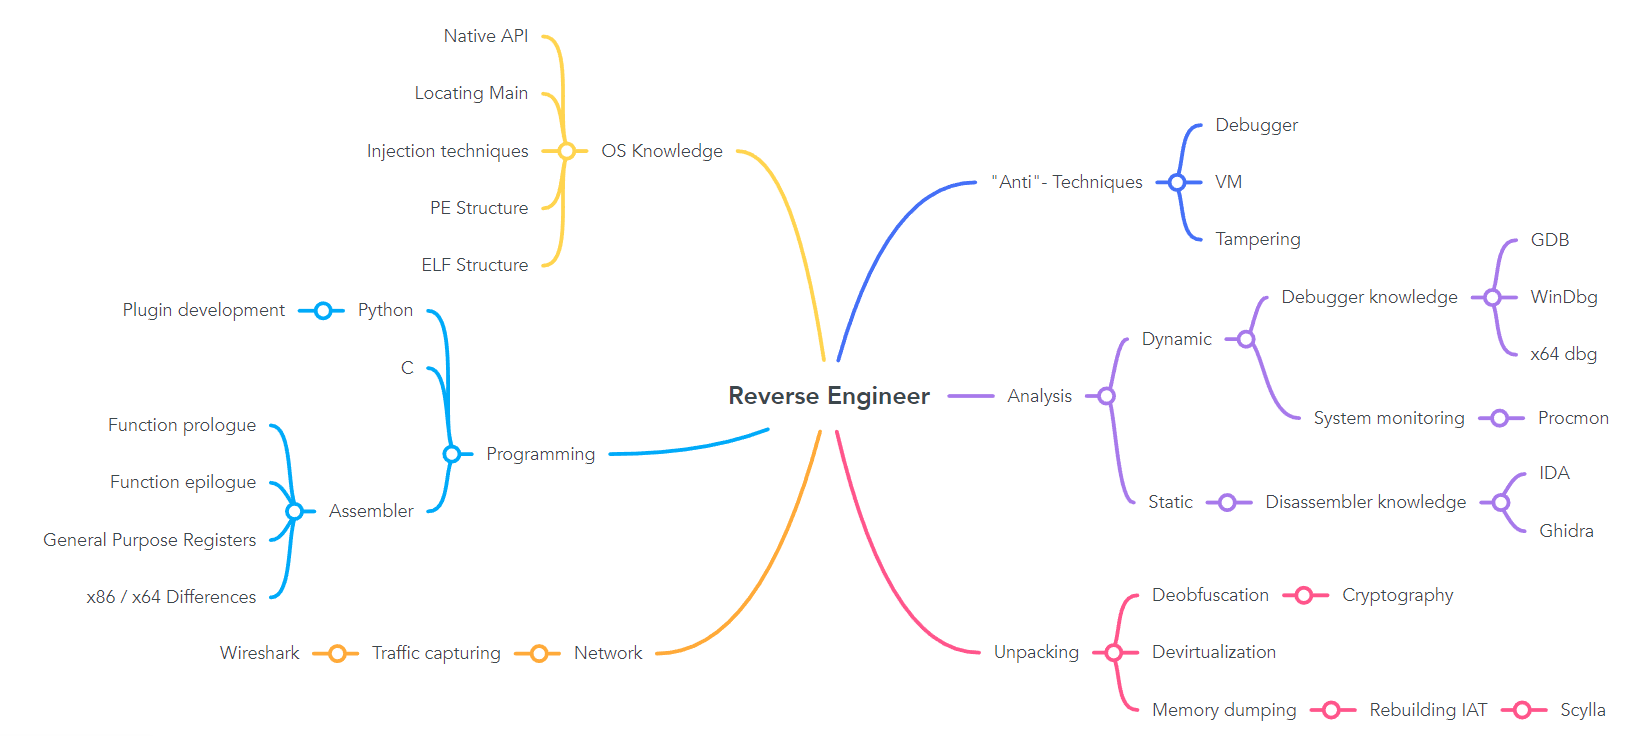
\includegraphics[height=250px, center]{resources/ReverseEngineeringDomain.png}
\section{Learning Concepts}
Based on the Problem Domain from the last section we decided the most basic domains were programming, analysis and OS knowledge. So we decided that we are going to create the most labs and the first ones about these topics and then the later introduce the other domains in later Labs. We want to focus on Linux and Windows.

We also decided that we can expect for Students to already know about C, Python and some basic knowledge about Assembler because everyone has to have had BSYS which teaches about Assembler and C. Automation with python is also a module which now is in every sample curriculum at the OST.

\begin{center}
    \begin{tabular}{ |p{3cm}|p{12cm}| } 
        \hline
            Topic & 
            Description \\ [0.5ex] 
        \hline
        \hline
            Debugging: Introduction & 
            We intend to first explain the diffrence between static and dynamic debugging. We also plan to introduce the programs we are going to use with download links and additional information of how to use them. We also have a fast repetition of the most important assembler topics (registers, functions).  \\ 
        \hline
            Static Debugging & 
            Here we will tackle the first program for Linux and open it up in Ghidra or IDA. We will also provide a sample code on which the program is based on. \\ 
        \hline
            Dynamic Debugging & 
            We will introduce the concept with the use of x64 dbg. In a simple excercise where you have to just patch some checks to get the flag. \\ 
        \hline
            Anti - Techniques & 
            We explain the Anti-Techniques and show examples of them and how to deal with them. \\ 
        \hline
            Unpacking & 
            We explain what Packing is, how to deal with it and specifically with devirtualization and deobfuscation. \\ 
        \hline
            Excercise Labs & 
            This is the final Lab/Labs in which the students can use everything they learned in the previous chapters to solve excercises in different difficulties. \\ 
        \hline
    \end{tabular}
\end{center}